%%%%%%%%%%%%%%%%%%%% author.tex %%%%%%%%%%%%%%%%%%%%%%%%%%%%%%%%%%%
%
% sample root file for your "contribution" to a contributed volume
%
% Use this file as a template for your own input.
%
%%%%%%%%%%%%%%%% Springer %%%%%%%%%%%%%%%%%%%%%%%%%%%%%%%%%%


% RECOMMENDED %%%%%%%%%%%%%%%%%%%%%%%%%%%%%%%%%%%%%%%%%%%%%%%%%%%
\documentclass[graybox]{svmult}

% choose options for [] as required from the list
% in the Reference Guide

\usepackage{mathptmx}       % selects Times Roman as basic font
\usepackage{helvet}         % selects Helvetica as sans-serif font
\usepackage{courier}        % selects Courier as typewriter font
\usepackage{type1cm}        % activate if the above 3 fonts are
                            % not available on your system
%
\usepackage{makeidx}         % allows index generation
\usepackage{graphicx}        % standard LaTeX graphics tool
                             % when including figure files
\usepackage{multicol}        % used for the two-column index
\usepackage[bottom]{footmisc}% places footnotes at page bottom

% see the list of further useful packages
% in the Reference Guide

\makeindex             % used for the subject index
                       % please use the style svind.ist with
                       % your makeindex program

%%%%%%%%%%%%%%%%%%%%%%%%%%%%%%%%%%%%%%%%%%%%%%%%%%%%%%%%%%%%%%%%%%%%%%%%%%%%%%%%%%%%%%%%%

\begin{document}

\title*{Robust disturbance estimator design for aircraft load alleviation control}
% Use \titlerunning{Short Title} for an abbreviated version of
% your contribution title if the original one is too long
\author{Daniel Ossmann and Charles Poussot-Vassal}
% Use \authorrunning{Short Title} for an abbreviated version of
% your contribution title if the original one is too long
\institute{Dr. Daniel Ossmann \at Institute of System Dynamics and Control, German Aerospace Center, Muenchener Strasse 20, 82234 Wessling, Germany, \email{daniel.ossmann@dlr.de}
\and Dr. Charles Poussot-Vassal \at Systems and Signal Processing Department, ONERA Centre de Toulouse, 2 Avenue Edouard Belin, 31000 Toulouse, France \email{Charles.Poussot-Vassal@onera.fr}}
%
% Use the package "url.sty" to avoid
% problems with special characters
% used in your e-mail or web address
%
\maketitle


%\abstract*{Each chapter should be preceded by an abstract (10--15 lines long) that summarizes the content. The abstract will appear \textit{online} at \url{www.SpringerLink.com} and be available with unrestricted access. This allows unregistered users to read the abstract as a teaser for the complete chapter. As a general rule the abstracts will not appear in the printed version of your book unless it is the style of your particular book or that of the series to which your book belongs. Please use the 'starred' version of the new Springer \texttt{abstract} command for typesetting the text of the online abstracts (cf. source file of this chapter template \texttt{abstract}) and include them with the source files of your manuscript. Use the plain \texttt{abstract} command if the abstract is also to appear in the printed version of the book.}

\abstract*{	In this paper a novel approach to design linear disturbance estimator is presented. The linear approach relies on the idea of directly decoupling everything but the disturbance input from the estimate by using advanced nullspace computation techniques. The main advantage of the approach is that disturbance estimators of minimal order, using available and numerically reliable tools, can be designed. The approach is applied to a generic model of a business jet aircraft. The derived disturbance estimate is used in a control algorithm to reduce the wing bending moments on the aircraft in case of wind gusts.
Both, the disturbance estimator together with the load alleviation controller are verified in a non-linear closed loop aircraft simulation model.}

\abstract{	In this paper a novel approach to design linear disturbance estimator is presented. The linear approach relies on the idea of directly decoupling everything but the disturbance input from the estimate by using advanced nullspace computation techniques. The main advantage of the approach is that disturbance estimators of minimal order, using available and numerically reliable tools, can be designed. The approach is applied to a generic model of a business jet aircraft. The derived disturbance estimate is used in a control algorithm to reduce the wing bending moments on the aircraft in case of wind gusts. Both, the disturbance estimator together with the load alleviation controller are verified in a non-linear closed loop aircraft simulation model.}



\section{Introduction}
%

\section{xxx}

\section{xxx}

\section{xxx}








\section*{Conclusions}




\begin{acknowledgement}
This work has been funded within the frame of the Joint Technology
Initiative JTI Clean Sky 2, AIRFRAME Integrated Technology Demonstrator
platform "AIRFRAME ITD" (contract N$^\circ$ CSJU-CS2-GAM-AIR-2014-15-01 Annex
1, Issue B04, October 2nd, 2015) being part of the Horizon 2020 research
and Innovation framework program of the European Commission.
\end{acknowledgement}
%
%\section*{Appendix}
%\addcontentsline{toc}{section}{Appendix}


%\input{referenc}
\end{document}

%%%%%%%%%%%%%%%%%%%%%%%%%%%%%%%%%%%%%%%%%%%%%%%%%%%%%%%%%%%%%%%%%%%%%%%%%%%%%%%%%%%%%%%%%%%%%%%%%%%%%%%%%%%%%%%%%%%%%%%%%%%%


%\begin{figure}[t]
%	\sidecaption[t]
%	% Use the relevant command for your figure-insertion program
%	% to insert the figure file.
%	% For example, with the option graphics use
%	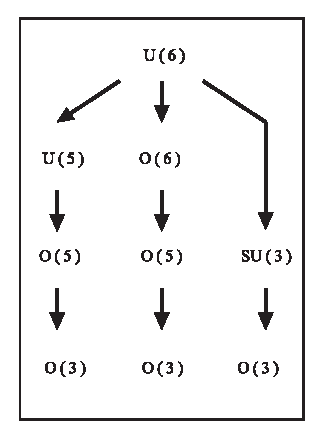
\includegraphics[scale=.65]{figure}
%	%
%	% If no graphics program available, insert a blank space i.e. use
%	%\picplace{5cm}{2cm} % Give the correct figure height and width in cm
%	%
%	%\caption{Please write your figure caption here}
%	\caption{If the width of the figure is less than 7.8 cm use the \texttt{sidecapion} command to flush the caption on the left side of the page. If the figure is positioned at the top of the page, align the sidecaption with the top of the figure -- to achieve this you simply need to use the optional argument \texttt{[t]} with the \texttt{sidecaption} command}
%	\label{fig:2}       % Give a unique label
%\end{figure}


%\begin{table}
%	\caption{Please write your table caption here}
%	\label{tab:1}       % Give a unique label
	%
%\begin{tabular}{p{2cm}p{2.4cm}p{2cm}p{4.9cm}}
%	\hline\noalign{\smallskip}
%	Classes & Subclass & Length & Action Mechanism  \\
%	\noalign{\smallskip}\svhline\noalign{\smallskip}
%	Translation & mRNA$^a$  & 22 (19--25) & Translation repression, mRNA cleavage\\
%	Translation & mRNA cleavage & 21 & mRNA cleavage\\
%	Translation & mRNA  & 21--22 & mRNA cleavage\\
%	Translation & mRNA  & 24--26 & Histone and DNA Modification\\
%	\noalign{\smallskip}\hline\noalign{\smallskip}
%\end{tabular}
%$^a$ Table foot note (with superscript)
%\end{table}


%\begin{svgraybox}
%If you want to emphasize complete paragraphs of texts we recommend to use the newly defined Springer class option \verb|graybox| and the newly defined environment \verb|svgraybox|. This will produce a 15 percent screened box 'behind' your text.
%
%If you want to emphasize complete paragraphs of texts we recommend to use the newly defined Springer class option and environment \verb|svgraybox|. This will produce a 15 percent screened box 'behind' your text.
%\end{svgraybox}


%
%\begin{proof}
%\smartqed
%Proof text goes here.
%\qed
%\end{proof}

%If you want to list definitions or the like we recommend to use the Springer-enhanced \verb|description| environment -- it will automatically render Springer's preferred layout.
%
%\begin{description}[Type 1]
%	\item[Type 1]{That addresses central themes pertainng to migration, health, and disease. In Sect.~\ref{sec:1}, Wilson discusses the role of human migration in infectious disease distributions and patterns.}
%	\item[Type 2]{That addresses central themes pertainng to migration, health, and disease. In Sect.~\ref{subsec:2}, Wilson discusses the role of human migration in infectious disease distributions and patterns.}
%\end{description}

%
